\documentclass{article}

% ---------------------------------------------------------------- %
% short package descriptions are copied from
% https://ctan.org/

% ---------------------------------------------------------------- %

% Accept different input encodings
\usepackage[utf8]{inputenc}

% Standard package for selecting font encodings
\usepackage[T1]{fontenc}

% ---------------------------------------------------------------- %

% Multilingual support for Plain TEX or LATEX
\usepackage[ngerman]{babel}

% ---------------------------------------------------------------- %

% Set all page margins to 1.5cm
\usepackage{fullpage}

% Margin adjustment and detection of odd/even pages
\usepackage{changepage}

% Flexible and complete interface to document dimensions
\usepackage{geometry}

% ---------------------------------------------------------------- %
% mathematics

\usepackage{amsmath}  % AMS mathematical facilities for LATEX
\usepackage{amssymb}
\usepackage{amsfonts} % TEX fonts from the American Mathematical Society
\usepackage{amsthm}   % Typesetting theorems (AMS style)

% Mathematical tools to use with amsmath
\usepackage{mathtools}

% Support for using RSFS fonts in maths
\usepackage{mathrsfs}

% Commands to produce dots in math that respect font size
\usepackage{mathdots}

% "Blackboard-style" cm fonts
\usepackage{bbm}

% Typeset in-line fractions in a "nice" way
\usepackage{nicefrac}

% Typeset quotient structures with LATEX
\usepackage{faktor}

% Vector arrows
\usepackage{esvect}

% St Mary Road symbols for theoretical computer science
\usepackage{stmaryrd}

% Three series of mathematical symbols
\usepackage{mathabx}

% ---------------------------------------------------------------- %
% algorithms

% Package for typesetting pseudocode
\usepackage{algpseudocode}

% Typeset source code listings using LATEX
\usepackage{listings}

% Reimplementation of and extensions to LATEX verbatim
\usepackage{verbatim}

% If necessary, please use the following 2 packages locally, but never both.
% This is because the algorithm environment gets defined in both packages, which leads to name conflicts.
% \usepackage{algorithm2e}
% \usepackage{algorithm}

% ---------------------------------------------------------------- %
% utilities

% A generic document command parser
\usepackage{xparse}

% Extended conditional commands
\usepackage{xifthen}

% e-TEX tools for LATEX
\usepackage{etoolbox}

% Define commands with suffixes
\usepackage{suffix}

% Extensive support for hypertext in LATEX
\usepackage{hyperref}

% Driver-independent color extensions for LATEX and pdfLATEX
\usepackage{xcolor}

% ---------------------------------------------------------------- %
% graphics

% -------------------------------- %

\usepackage{tikz}

% MISC
\usetikzlibrary{patterns}
\usetikzlibrary{decorations.markings}
\usetikzlibrary{positioning}
\usetikzlibrary{arrows}
\usetikzlibrary{arrows.meta}
\usetikzlibrary{overlay-beamer-styles}

% finite state machines
\usetikzlibrary{automata}

% turing machines
\usetikzlibrary{calc}
\usetikzlibrary{chains}
\usetikzlibrary{decorations.pathmorphing}

% -------------------------------- %

% Draw tree structures
\usepackage[noeepic]{qtree}

% Enhanced support for graphics
\usepackage{graphicx}

% Figures broken into subfigures
\usepackage{subfig}

% Improved interface for floating objects
\usepackage{float}

% Control float placement
\usepackage{placeins}

% Include PDF documents in LATEX
\usepackage{pdfpages}

% ---------------------------------------------------------------- %

% Control layout of itemize, enumerate, description
\usepackage[inline]{enumitem}

% Intermix single and multiple columns
\usepackage{multicol}
\setlength{\columnsep}{1cm}

% Coloured boxes, for LATEX examples and theorems, etc
\usepackage{tcolorbox}

% ---------------------------------------------------------------- %
% tables

% Tabulars with adjustable-width columns
\usepackage{tabularx}

% Tabular column heads and multilined cells
\usepackage{makecell}

% Publication quality tables in LATEX
\usepackage{booktabs}

% ---------------------------------------------------------------- %
% bibliography and quoting

% Sophisticated Bibliographies in LATEX
\usepackage[backend = biber, style = alphabetic]{biblatex}

% Context sensitive quotation facilities
\usepackage{csquotes}

% ---------------------------------------------------------------- %

% ---------------------------------------------------------------- %
% special letters

\newcommand{\N}{\mathbb N}
\newcommand{\Z}{\mathbb Z}
\newcommand{\Q}{\mathbb Q}
\newcommand{\R}{\mathbb R}
\newcommand{\C}{\mathbb C}
\newcommand{\K}{\mathbb K}
\newcommand{\T}{\mathbb T}
\newcommand{\E}{\mathbb E}
\newcommand{\V}{\mathbb V}
\renewcommand{\S}{\mathbb S}
\renewcommand{\P}{\mathbb P}
\newcommand{\1}{\mathbbm 1}
\newcommand{\G}{\mathbb G}

\newcommand{\iu}{\mathrm i}

% ---------------------------------------------------------------- %
% quantors

\newcommand{\Forall}        {\forall ~}
\newcommand{\Exists}        {\exists ~}
\newcommand{\nExists}       {\nexists ~}
\newcommand{\ExistsOnlyOne} {\exists! ~}
\newcommand{\nExistsOnlyOne}{\nexists! ~}
\newcommand{\ForAlmostAll}  {\forall^\infty ~}

% ---------------------------------------------------------------- %
% graphics boxed

\newcommand
{\includegraphicsboxed}
[2][0.75]
{
    \begin{center}
        \begin{tcolorbox}[standard jigsaw, opacityback = 0]

            \centering
            \includegraphics[width = #1 \textwidth]{#2}

        \end{tcolorbox}
    \end{center}
}

\newcommand
{\includegraphicsunboxed}
[2][0.75]
{
    \begin{center}
        \includegraphics[width = #1 \textwidth]{#2}
    \end{center}
}

\NewDocumentCommand
{\includegraphicsgraphicsboxed}
{ O{0.75} O{0.25} m m}
{
    \begin{center}
        \begin{tcolorbox}[standard jigsaw, opacityback = 0]

            \centering
            \includegraphics[width = #1 \textwidth]{#3} \\
            \vspace{#2 cm}
            \includegraphics[width = #1 \textwidth]{#4}

        \end{tcolorbox}
    \end{center}
}

\NewDocumentCommand
{\includegraphicsgraphicsunboxed}
{ O{0.75} O{0.25} m m}
{
    \begin{center}

        \centering
        \includegraphics[width = #1 \textwidth]{#3} \\
        \vspace{#2 cm}
        \includegraphics[width = #1 \textwidth]{#4}

    \end{center}
}

% ---------------------------------------------------------------- %
% braces

\newcommand{\pbraces}[1]{{\left  ( #1 \right  )}}
\newcommand{\bbraces}[1]{{\left  [ #1 \right  ]}}
\newcommand{\Bbraces}[1]{{\left \{ #1 \right \}}}
\newcommand{\vbraces}[1]{{\left  | #1 \right  |}}
\newcommand{\Vbraces}[1]{{\left \| #1 \right \|}}

\newcommand{\abraces}[1]{{\left \langle #1 \right \rangle}}

\newcommand{\floorbraces}[1]{{\left \lfloor #1 \right \rfloor}}
\newcommand{\ceilbraces} [1]{{\left \lceil  #1 \right \rceil }}

\newcommand{\dbbraces}    [1]{{\llbracket     #1 \rrbracket}}
\newcommand{\dpbraces}    [1]{{\llparenthesis #1 \rrparenthesis}}
\newcommand{\dfloorbraces}[1]{{\llfloor       #1 \rrfloor}}
\newcommand{\dceilbraces} [1]{{\llceil        #1 \rrceil}}

\newcommand{\dabraces}[1]{{\left \langle \left \langle #1 \right \rangle \right \rangle}}

\newcommand{\abs}  [1]{\vbraces{#1}}
\newcommand{\round}[1]{\bbraces{#1}}
\newcommand{\floor}[1]{\floorbraces{#1}}
\newcommand{\ceil} [1]{\ceilbraces{#1}}

% ---------------------------------------------------------------- %

% MISC

% metric spaces
\newcommand{\norm}[2][]{\Vbraces{#2}_{#1}}
\DeclareMathOperator{\metric}{d}
\DeclareMathOperator{\dist}  {dist}
\DeclareMathOperator{\diam}  {diam}

% O-notation
\newcommand{\landau}{{\scriptstyle \mathcal{O}}}
\newcommand{\Landau}{\mathcal{O}}

% ---------------------------------------------------------------- %

% math operators

% hyperbolic trigonometric function inverses
\DeclareMathOperator{\areasinh}{areasinh}
\DeclareMathOperator{\areacosh}{areacosh}
\DeclareMathOperator{\areatanh}{areatanh}

% special functions
\DeclareMathOperator{\id} {id}
\DeclareMathOperator{\sgn}{sgn}
\DeclareMathOperator{\Inv}{Inv}
\DeclareMathOperator{\erf}{erf}
\DeclareMathOperator{\pv} {pv}

% exponential function as power
\WithSuffix \newcommand \exp* [1]{\mathrm{e}^{#1}}

% operations on sets
\DeclareMathOperator{\meas}{meas}
\DeclareMathOperator{\card}{card}
\DeclareMathOperator{\Span}{span}
\DeclareMathOperator{\conv}{conv}
\DeclareMathOperator{\cof}{cof}
\DeclareMathOperator{\mean}{mean}
\DeclareMathOperator{\avg}{avg}
\DeclareMathOperator*{\argmax}{argmax}
\DeclareMathOperator*{\argsmax}{argsmax}

% number theory stuff
\DeclareMathOperator{\ggT}{ggT}
\DeclareMathOperator{\kgV}{kgV}
\DeclareMathOperator{\modulo}{mod}

% polynomial stuff
\DeclareMathOperator{\ord}{ord}
\DeclareMathOperator{\grad}{grad}

% function properties
\DeclareMathOperator{\ran}{ran}
\DeclareMathOperator{\supp}{supp}
\DeclareMathOperator{\graph}{graph}
\DeclareMathOperator{\dom}{dom}
\DeclareMathOperator{\Def}{def}
\DeclareMathOperator{\rg}{rg}

% matrix stuff
\DeclareMathOperator{\GL}{GL}
\DeclareMathOperator{\SL}{SL}
\DeclareMathOperator{\U}{U}
\DeclareMathOperator{\SU}{SU}
\DeclareMathOperator{\PSU}{PSU}
% \DeclareMathOperator{\O}{O}
% \DeclareMathOperator{\PO}{PO}
% \DeclareMathOperator{\PSO}{PSO}
\DeclareMathOperator{\diag}{diag}

% algebra stuff
\DeclareMathOperator{\At}{At}
\DeclareMathOperator{\Ob}{Ob}
\DeclareMathOperator{\Hom}{Hom}
\DeclareMathOperator{\End}{End}
\DeclareMathOperator{\Aut}{Aut}
\DeclareMathOperator{\Lin}{L}

% other function classes
\DeclareMathOperator{\Lip}{Lip}
\DeclareMathOperator{\Mod}{Mod}
\DeclareMathOperator{\Dil}{Dil}

% constants
\DeclareMathOperator{\NIL}{NIL}
\DeclareMathOperator{\eps}{eps}

% ---------------------------------------------------------------- %
% doubble & tripple powers

\newcommand
{\primeprime}
{{\prime \prime}}

\newcommand
{\primeprimeprime}
{{\prime \prime \prime}}

\newcommand
{\astast}
{{\ast \ast}}

\newcommand
{\astastast}
{{\ast \ast \ast}}

% ---------------------------------------------------------------- %
% derivatives

\NewDocumentCommand
{\derivative}
{ O{} O{} m m}
{
    \frac
    {\mathrm d^{#2} {#1}}
    {\mathrm d {#3}^{#2}}
}

\NewDocumentCommand
{\pderivative}
{ O{} O{} m m}
{
    \frac
    {\partial^{#2} {#1}}
    {\partial {#3}^{#2}}
}

\DeclareMathOperator{\Div}{div}
\DeclareMathOperator{\rot}{rot}

% ---------------------------------------------------------------- %
% integrals

\NewDocumentCommand
{\Int}
{ O{} O{} m m}
{\int_{#1}^{#2} #3 ~ \mathrm d #4}

\NewDocumentCommand
{\Iint}
{ O{} O{} m m m}
{\iint_{#1}^{#2} #3 ~ \mathrm d #4 ~ \mathrm d #5}

\NewDocumentCommand
{\Iiint}
{ O{} O{} m m m m}
{\iiint_{#1}^{#2} #3 ~ \mathrm d #4 ~ \mathrm d #5 ~ \mathrm d #6}

\NewDocumentCommand
{\Iiiint}
{ O{} O{} m m m m m}
{\iiiint_{#1}^{#2} #3 ~ \mathrm d #4 ~ \mathrm d #5 ~ \mathrm d #6 ~ \mathrm d #7}

\NewDocumentCommand
{\Idotsint}
{ O{} O{} m m m}
{\idotsint_{#1}^{#2} #3 ~ \mathrm d #4 \dots ~ \mathrm d #5}

\NewDocumentCommand
{\Oint}
{ O{} O{} m m}
{\oint_{#1}^{#2} #3 ~ \mathrm d #4}

% ---------------------------------------------------------------- %

% source:
% https://tex.stackexchange.com/questions/203257/tikz-chains-with-one-side-of-the-leftmost-node-thickbold

% #1 (optional): current state, e.g. $q_0$
% #2: cursor position, e.g. 1
% #3: number of displayed cells, e.g. 5
% #4: contents of cells, e.g. {$\triangleright$, $x_1$, \dots, $x_n$, \textvisiblespace}

\newcommand{\turingtape}[4][]
{
    \begin{tikzpicture}

        \tikzset{tape/.style={minimum size=.7cm, draw}}

        \begin{scope}[start chain=0 going right, node distance=0mm]
            \foreach \x [count=\i] in #4
            {
                \ifnum\i=#3 % if last node reset outer sep to 0pt
                    \node [on chain=0, tape, outer sep=0pt] (n\i) {\x};
                    \draw (n\i.north east) -- ++(.1,0) decorate [decoration={zigzag, segment length=.12cm, amplitude=.02cm}] {-- ($(n\i.south east)+(+.1,0)$)} -- (n\i.south east) -- cycle;
                \else
                    \node [on chain=0, tape] (n\i) {\x};
                \fi

                \ifnum\i=1 % if first node draw a thick line at the left
                    \draw [line width=.1cm] (n\i.north west) -- (n\i.south west);
                \fi
            }
 
            \node [right=.25cm of n#3] {$\cdots$};
            \node [tape, above left=.25cm and 1cm of n1] (q) {#1};
            \draw [>=latex, ->] (q) -| (n#2);

        \end{scope}

    \end{tikzpicture}
}

% ---------------------------------------------------------------- %

% ---------------------------------------------------------------- %
% amsthm-environments:

\theoremstyle{definition}

% numbered theorems
\newtheorem{theorem}             {Satz}[section]
\newtheorem{lemma}      [theorem]{Lemma}
\newtheorem{corollary}  [theorem]{Korollar}
\newtheorem{proposition}[theorem]{Proposition}
\newtheorem{remark}     [theorem]{Bemerkung}
\newtheorem{definition} [theorem]{Definition}
\newtheorem{example}    [theorem]{Beispiel}
\newtheorem{heuristics} [theorem]{Heuristik}

% unnumbered theorems
\newtheorem*{theorem*}    {Satz}
\newtheorem*{lemma*}      {Lemma}
\newtheorem*{corollary*}  {Korollar}
\newtheorem*{proposition*}{Proposition}
\newtheorem*{remark*}     {Bemerkung}
\newtheorem*{definition*} {Definition}
\newtheorem*{example*}    {Beispiel}
\newtheorem*{heuristics*} {Heuristik}

% ---------------------------------------------------------------- %
% exercise- and solution-environments:

% Please define this stuff in project ("main.tex"):
% \def \lastexercisenumber {...}

\newtheorem{exercise}{Aufgabe}
\setcounter{exercise}{\lastexercisenumber}

\newenvironment{solution}
{
  \begin{proof}[Lösung]
}{
  \end{proof}
}

% ---------------------------------------------------------------- %
% MISC translations for environment-names

\renewcommand{\proofname} {Beweis}
\renewcommand{\figurename}{Abbildung}
\renewcommand{\tablename} {Tabelle}

% ---------------------------------------------------------------- %

% ---------------------------------------------------------------- %
% https://www.overleaf.com/learn/latex/Code_listing

\definecolor{codegreen} {rgb}{0, 0.6, 0}
\definecolor{codegray}    {rgb}{0.5, 0.5, 0.5}
\definecolor{codepurple}{rgb}{0.58, 0, 0.82}
\definecolor{backcolour}{rgb}{0.95, 0.95, 0.92}

\lstdefinestyle{overleaf}
{
    backgroundcolor = \color{backcolour},
    commentstyle = \color{codegreen},
    keywordstyle = \color{magenta},
    numberstyle = \tiny\color{codegray},
    stringstyle = \color{codepurple},
    basicstyle = \ttfamily \footnotesize,
    breakatwhitespace = false,
    breaklines = true,
    captionpos = b,
    keepspaces = true,
    numbers = left,
    numbersep = 5pt,
    showspaces = false,
    showstringspaces = false,
    showtabs = false,
    tabsize = 2
}

% ---------------------------------------------------------------- %
% https://en.wikibooks.org/wiki/LaTeX/Source_Code_Listings

\lstdefinestyle{customc}
{
    belowcaptionskip = 1 \baselineskip,
    breaklines = true,
    frame = L,
    xleftmargin = \parindent,
    language = C,
    showstringspaces = false,
    basicstyle = \footnotesize \ttfamily,
    keywordstyle = \bfseries \color{green!40!black},
    commentstyle = \itshape \color{purple!40!black},
    identifierstyle = \color{blue},
    stringstyle = \color{orange},
}

\lstdefinestyle{customasm}
{
    belowcaptionskip = 1 \baselineskip,
    frame = L,
    xleftmargin = \parindent,
    language = [x86masm] Assembler,
    basicstyle = \footnotesize\ttfamily,
    commentstyle = \itshape\color{purple!40!black},
}

% ---------------------------------------------------------------- %
% https://tex.stackexchange.com/questions/235731/listings-syntax-for-literate

\definecolor{maroon}        {cmyk}{0, 0.87, 0.68, 0.32}
\definecolor{halfgray}      {gray}{0.55}
\definecolor{ipython_frame} {RGB}{207, 207, 207}
\definecolor{ipython_bg}    {RGB}{247, 247, 247}
\definecolor{ipython_red}   {RGB}{186, 33, 33}
\definecolor{ipython_green} {RGB}{0, 128, 0}
\definecolor{ipython_cyan}  {RGB}{64, 128, 128}
\definecolor{ipython_purple}{RGB}{170, 34, 255}

\lstdefinestyle{stackexchangePython}
{
    breaklines = true,
    %
    extendedchars = true,
    literate =
    {á}{{\' a}} 1 {é}{{\' e}} 1 {í}{{\' i}} 1 {ó}{{\' o}} 1 {ú}{{\' u}} 1
    {Á}{{\' A}} 1 {É}{{\' E}} 1 {Í}{{\' I}} 1 {Ó}{{\' O}} 1 {Ú}{{\' U}} 1
    {à}{{\` a}} 1 {è}{{\` e}} 1 {ì}{{\` i}} 1 {ò}{{\` o}} 1 {ù}{{\` u}} 1
    {À}{{\` A}} 1 {È}{{\' E}} 1 {Ì}{{\` I}} 1 {Ò}{{\` O}} 1 {Ù}{{\` U}} 1
    {ä}{{\" a}} 1 {ë}{{\" e}} 1 {ï}{{\" i}} 1 {ö}{{\" o}} 1 {ü}{{\" u}} 1
    {Ä}{{\" A}} 1 {Ë}{{\" E}} 1 {Ï}{{\" I}} 1 {Ö}{{\" O}} 1 {Ü}{{\" U}} 1
    {â}{{\^ a}} 1 {ê}{{\^ e}} 1 {î}{{\^ i}} 1 {ô}{{\^ o}} 1 {û}{{\^ u}} 1
    {Â}{{\^ A}} 1 {Ê}{{\^ E}} 1 {Î}{{\^ I}} 1 {Ô}{{\^ O}} 1 {Û}{{\^ U}} 1
    {œ}{{\oe}}  1 {Œ}{{\OE}}  1 {æ}{{\ae}}  1 {Æ}{{\AE}}  1 {ß}{{\ss}}  1
    {ç}{{\c c}} 1 {Ç}{{\c C}} 1 {ø}{{\o}} 1 {å}{{\r a}} 1 {Å}{{\r A}} 1
    {€}{{\EUR}} 1 {£}{{\pounds}} 1
}


% Python definition (c) 1998 Michael Weber
% Additional definitions (2013) Alexis Dimitriadis
% modified by me (should not have empty lines)

\lstdefinelanguage{iPython}{
    morekeywords = {access, and, break, class, continue, def, del, elif, else, except, exec, finally, for, from, global, if, import, in, is, lambda, not, or, pass, print, raise, return, try, while}, %
    %
    % Built-ins
    morekeywords = [2]{abs, all, any, basestring, bin, bool, bytearray, callable, chr, classmethod, cmp, compile, complex, delattr, dict, dir, divmod, enumerate, eval, execfile, file, filter, float, format, frozenset, getattr, globals, hasattr, hash, help, hex, id, input, int, isinstance, issubclass, iter, len, list, locals, long, map, max, memoryview, min, next, object, oct, open, ord, pow, property, range, raw_input, reduce, reload, repr, reversed, round, set, setattr, slice, sorted, staticmethod, str, sum, super, tuple, type, unichr, unicode, vars, xrange, zip, apply, buffer, coerce, intern}, %
    %
    sensitive = true, %
    morecomment = [l] \#, %
    morestring = [b]', %
    morestring = [b]", %
    %
    morestring = [s]{'''}{'''}, % used for documentation text (mulitiline strings)
    morestring = [s]{"""}{"""}, % added by Philipp Matthias Hahn
    %
    morestring = [s]{r'}{'},     % `raw' strings
    morestring = [s]{r"}{"},     %
    morestring = [s]{r'''}{'''}, %
    morestring = [s]{r"""}{"""}, %
    morestring = [s]{u'}{'},     % unicode strings
    morestring = [s]{u"}{"},     %
    morestring = [s]{u'''}{'''}, %
    morestring = [s]{u"""}{"""}, %
    %
    % {replace}{replacement}{lenght of replace}
    % *{-}{-}{1} will not replace in comments and so on
    literate = 
    {á}{{\' a}} 1 {é}{{\' e}} 1 {í}{{\' i}} 1 {ó}{{\' o}} 1 {ú}{{\' u}} 1
    {Á}{{\' A}} 1 {É}{{\' E}} 1 {Í}{{\' I}} 1 {Ó}{{\' O}} 1 {Ú}{{\' U}} 1
    {à}{{\` a}} 1 {è}{{\` e}} 1 {ì}{{\` i}} 1 {ò}{{\` o}} 1 {ù}{{\` u}} 1
    {À}{{\` A}} 1 {È}{{\' E}} 1 {Ì}{{\` I}} 1 {Ò}{{\` O}} 1 {Ù}{{\` U}} 1
    {ä}{{\" a}} 1 {ë}{{\" e}} 1 {ï}{{\" i}} 1 {ö}{{\" o}} 1 {ü}{{\" u}} 1
    {Ä}{{\" A}} 1 {Ë}{{\" E}} 1 {Ï}{{\" I}} 1 {Ö}{{\" O}} 1 {Ü}{{\" U}} 1
    {â}{{\^ a}} 1 {ê}{{\^ e}} 1 {î}{{\^ i}} 1 {ô}{{\^ o}} 1 {û}{{\^ u}} 1
    {Â}{{\^ A}} 1 {Ê}{{\^ E}} 1 {Î}{{\^ I}} 1 {Ô}{{\^ O}} 1 {Û}{{\^ U}} 1
    {œ}{{\oe}}  1 {Œ}{{\OE}}  1 {æ}{{\ae}}  1 {Æ}{{\AE}}  1 {ß}{{\ss}}  1
    {ç}{{\c c}} 1 {Ç}{{\c C}} 1 {ø}{{\o}} 1 {å}{{\r a}} 1 {Å}{{\r A}} 1
    {€}{{\EUR}} 1 {£}{{\pounds}} 1
    %
    {^}{{{\color{ipython_purple}\^ {}}}} 1
    { = }{{{\color{ipython_purple} = }}} 1
    %
    {+}{{{\color{ipython_purple}+}}} 1
    {*}{{{\color{ipython_purple}$^\ast$}}} 1
    {/}{{{\color{ipython_purple}/}}} 1
    %
    {+=}{{{+=}}} 1
    {-=}{{{-=}}} 1
    {*=}{{{$^\ast$ = }}} 1
    {/=}{{{/=}}} 1,
    literate = 
    *{-}{{{\color{ipython_purple} -}}} 1
     {?}{{{\color{ipython_purple} ?}}} 1,
    %
    identifierstyle = \color{black}\ttfamily,
    commentstyle = \color{ipython_cyan}\ttfamily,
    stringstyle = \color{ipython_red}\ttfamily,
    keepspaces = true,
    showspaces = false,
    showstringspaces = false,
    %
    rulecolor = \color{ipython_frame},
    frame = single,
    frameround = {t}{t}{t}{t},
    framexleftmargin = 6mm,
    numbers = left,
    numberstyle = \tiny\color{halfgray},
    %
    %
    backgroundcolor = \color{ipython_bg},
    % extendedchars = true,
    basicstyle = \scriptsize,
    keywordstyle = \color{ipython_green}\ttfamily,
}

% ---------------------------------------------------------------- %
% https://tex.stackexchange.com/questions/417884/colour-r-code-to-match-knitr-theme-using-listings-minted-or-other

\geometry{verbose, tmargin = 2.5cm, bmargin = 2.5cm, lmargin = 2.5cm, rmargin = 2.5cm}

\definecolor{backgroundCol}  {rgb}{.97, .97, .97}
\definecolor{commentstyleCol}{rgb}{0.678, 0.584, 0.686}
\definecolor{keywordstyleCol}{rgb}{0.737, 0.353, 0.396}
\definecolor{stringstyleCol} {rgb}{0.192, 0.494, 0.8}
\definecolor{NumCol}         {rgb}{0.686, 0.059, 0.569}
\definecolor{basicstyleCol}  {rgb}{0.345, 0.345, 0.345}

\lstdefinestyle{stackexchangeR}
{
    language = R,                                        % the language of the code
    basicstyle = \small \ttfamily \color{basicstyleCol}, % the size of the fonts that are used for the code
    % numbers = left,                                      % where to put the line-numbers
    numberstyle = \color{green},                         % the style that is used for the line-numbers
    stepnumber = 1,                                      % the step between two line-numbers. If it is 1, each line will be numbered
    numbersep = 5pt,                                     % how far the line-numbers are from the code
    backgroundcolor = \color{backgroundCol},             % choose the background color. You must add \usepackage{color}
    showspaces = false,                                  % show spaces adding particular underscores
    showstringspaces = false,                            % underline spaces within strings
    showtabs = false,                                    % show tabs within strings adding particular underscores
    % frame = single,                                      % adds a frame around the code
    % rulecolor = \color{white},                           % if not set, the frame-color may be changed on line-breaks within not-black text (e.g. commens (green here))
    tabsize = 2,                                         % sets default tabsize to 2 spaces
    captionpos = b,                                      % sets the caption-position to bottom
    breaklines = true,                                   % sets automatic line breaking
    breakatwhitespace = false,                           % sets if automatic breaks should only happen at whitespace
    keywordstyle = \color{keywordstyleCol},              % keyword style
    commentstyle = \color{commentstyleCol},              % comment style
    stringstyle = \color{stringstyleCol},                % string literal style
    literate = %
    *{0}{{{\color{NumCol} 0}}} 1
     {1}{{{\color{NumCol} 1}}} 1
     {2}{{{\color{NumCol} 2}}} 1
     {3}{{{\color{NumCol} 3}}} 1
     {4}{{{\color{NumCol} 4}}} 1
     {5}{{{\color{NumCol} 5}}} 1
     {6}{{{\color{NumCol} 6}}} 1
     {7}{{{\color{NumCol} 7}}} 1
     {8}{{{\color{NumCol} 8}}} 1
     {9}{{{\color{NumCol} 9}}} 1
}

% ---------------------------------------------------------------- %
% Fundament Mathematik

\lstdefinestyle{fundament}{basicstyle = \ttfamily}

% ---------------------------------------------------------------- %


\addbibresource{../../../Fundament-LaTeX/references.bib}

\graphicspath{{../../../Fundament-LaTeX/images/}}

\parskip 0pt
\parindent 0pt

\title
{
  Diskrete und Geometrische Algorithmen \\
  \vspace{4pt}
  \normalsize
  \textit{3. Übung am 9.11.2020}
}
\author
{
  Richard Weiss
  \and
  Florian Schager
  \and
  Christian Sallinger
  \and
  Fabian Zehetgruber
  \and
  Paul Winkler
  \and
  Christian Göth
}
\date{}

\setcounter{exercise}{12}

\begin{document}

\maketitle

% --------------------------------------------------------------------------------

\begin{exercise}

Gegeben sei ein zusammenhängender ungerichteter Graph $G = (V,E)$ mit einer geraden Anzahl an Knoten.
Zeigen Sie, dass es einen (nicht notwendigerweise zusammenhängenden) Untergraph mit
Knotenmenge $V$ gibt (also einen Graph $G^\prime = (V, E^\prime)$ mit $E^\prime \subseteq E$),
in dem alle Knotengrade ungerade sind.

(Hinweis: beweisen Sie die Behauptung für Bäume und begründen Sie, warum diese Annahme reicht.)

\end{exercise}

% --------------------------------------------------------------------------------

\begin{solution}
Der Grad eines Knoten $v \in V$
ist definert als $\grad(x) = |\{\{x,y\}: \{x,y\} \in E\}|$. \\
Wir beweisen die Aussage mit Induktion nach $n := |V|$: \\
Für $n = 2$ gibt es genau eine Kante, welche die beiden Knoten verbindet,
also gilt die Aussage bereits für $E^{\prime} = E$. \\
Induktionsschritt: $n \rightsquigarrow n + 2$: \\
Betrachte einen beliebigen Baum $G$ mit $V = \{x_1,\dots,x_{n+2}\}$.
Nun existiert ein $v \in V$ mit $\grad(v) = 1$ (o.B.d.A. $v = x_{n+2}$).
Nun ist $G_1 = (V_1,E_1)$ mit
\begin{align*}
  V_1 &:= \{x_1,\dots,x_{n+1}\} \\
  E_1 &:= \{\{x,y\} \in E: x,y \in V_1\}
\end{align*}
klarerweise immer noch zyklenfrei und zusammenhängend und wir können
ein weiteres $v \in V_1$ mit $\grad(v) = 1$ (o.B.d.A: $v = x_{n+1}$) finden, sodass
dann $G = (V_2,E_2)$ mit
\begin{align*}
  V_2 &:= \{x_1,\dots,x_{n}\} \\
    E_1 &:= \{\{x,y\} \in E: x,y \in V_2\}
\end{align*}
ein zusammenhängender, zyklenfreier Graph ist, auf den wir die Induktionsvoraussetzung
anwenden können, also erhalten wir $E_2^{\prime} \subseteq E_2$, sodass
für alle $v \in V_2: \grad(v) = 1$. \\
Nun definieren wir $E^{\prime} = E_2^{\prime} \cup \{\{x_n,x_{n+1}\}\}$, welches
die Bedingung dann für alle $v \in V$ erfüllt. \\


Für einen beliebig zusammenhängenden Graphen $G = (V,E)$ mit gerader Knotenanzahl
erinnern wir uns daran, dass
ein Baum genau ein minimal zusammenhängender Graph ist.
Also finden wir in jedem Fall ein $E_1 \subseteq E$, sodass $G_1 = (V,E_1)$
ein Baum ist und wir das soeben gezeigte anwenden können.
\end{solution}

% --------------------------------------------------------------------------------

% -------------------------------------------------------------------------------- %

\begin{exercise}

Formulieren und beweisen Sie das Lemma $3.8$ explizit für den Fall $m=2$.

\end{exercise}

% -------------------------------------------------------------------------------- %

\begin{solution}

\begin{figure}[h!]
  \centering
  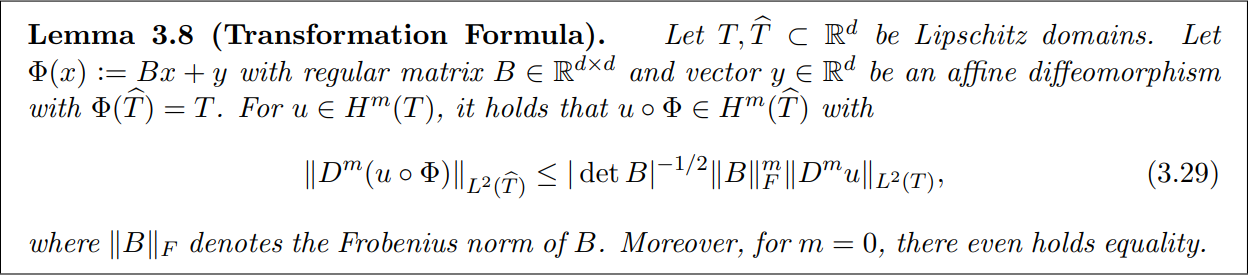
\includegraphics
  [width = 0.75 \textwidth]
  {NumPDEs/NumPDEs - Lemma 3.8 (Transformation Formula).png}
\end{figure}

\begin{align*}
  \Psi:
  C^\infty(\overline T) \to H^2(\hat T):
  u \mapsto u \circ \Phi
\end{align*}

Wir zeigen zuerst die Wohldefiniertheit von $\Psi$ als linearer und
beschränkter Operator, d.h. $\Exists C > 0:$

\begin{align*}
  \norm[H^2(\hat T)]{\Psi u}
  \leq
  C \norm[H^2(T)]{u}.
\end{align*}

Dazu zeigen wir zunächst die Transformationsfomel für $u \in C^{\infty}(\overline{T})$ und $m = 0,1,2$.

\begin{enumerate}[label = \arabic*.]

  \item Abschätzung ($m = 0$):
  Die steht sogar explizit im Skript.

  \begin{align*}
    \implies
    \norm[L^2(T)]{u}^2
    =
    \Int[T]{u^2}{y}
    =
    \Int[\hat T]{(u \circ \Phi)^2 |\det D \Phi|}{x}
    =
    |\det B| \norm[L^2(\hat T)]{u \circ \Phi}^2
  \end{align*}

  \item Abschätzung ($m = 1$):

  \begin{align*}
    \implies
    \partial_j (u \circ \Phi)(x)
    =
    \sum_{n=1}^d
    \partial_n u(\Phi(x)) B_{nj}
  \end{align*}

  Jetzt verwenden wir die Cauchy-Schwarz-Bunjakovski Ungleichung.

  \begin{align*}
    \implies
    |\partial_j (u \circ \Phi)(x)|^2
    & \stackrel
    {
      \mathrm{CSB}
    }
    {\leq}
    \pbraces
    {
      \sum_{n=1}^d
      \partial_n u(\Phi(x))|^2
    }
    \pbraces
    {
      \sum_{n=1}^d
      B_{nj}^2
    }
    =
    |Du(\Phi(x))|^2
    \pbraces
    {
      \sum_{n=1}^d
      B_{nj}^2
    }
    \end{align*}

  Jetzt verwenden wir die Transformationsfomel.

  \begin{align*}
    \implies
    |\det B| \norm[L^2(\hat T)]{D(u \circ \Phi)}^2
    & =
    \Int[\hat T]
    {
      \sum_{j=1}^d
      |\partial_j (u \circ \Phi)(x)|^2
      |\det D \Phi(x)|
    }{x} \\
    & \leq
    \Int[\hat T]
    {
      \sum_{j=1}^d
      |Du(\Phi(x))|^2
      \pbraces
      {
        \sum_{n=1}^d
        B_{nj}^2
      }
      |\det D \Phi(x)|
    }{x} \\
    & =
    \sum_{j=1}^d
    \pbraces
    {
      \sum_{n=1}^d
      B_{nj}^2
    }
    \Int[\hat T]
    {
      |Du(\Phi(x))|^2
      |\det D \Phi(x)|
      }{x} \\
    & \stackrel
    {
      \mathrm{TRAFO}
    }{=}
    \sum_{j=1}^d
    \pbraces
    {
      \sum_{n=1}^d
      B_{nj}^2
    }
    \Int[T]
    {
      |Du(x)|^2
    }{x} \\
    & =
    \norm[F]{B}^2 \norm[L^2(T)]{Du}^2
  \end{align*}

  \item Abschätzung ($m = 2$):

  \begin{align*}
    \implies
    D(u \circ \Phi) = Du(\Phi(x))D\Phi(x) = Du(\Phi(x))B
  \end{align*}

  \begin{align*}
    \implies
    \partial_k \partial_j (u \circ \Phi)(x)
    &=
    \partial_k \pbraces
    {
      \sum_{n=1}^d
      \partial_n u(\Phi(x)) B_{nj}
    } \\
    &=
    \sum_{n=1}^d
    B_{nj} \partial_k (\partial_n u(\Phi(x)))
    =
    \sum_{n=1}^d
    \sum_{m=1}^d
    \partial_m \partial_n u(\Phi(x)) B_{nj} B_{mk}
  \end{align*}

  Jetzt verwenden wir Cauchy-Schwarz-Bunjakovski.

  \begin{align*}
    \implies
    |\partial_k \partial_j (u \circ \Phi)(x)|^2
    &\stackrel
    {
      \mathrm{CSB}
    }
    {\leq}
    \pbraces
    {
      \sum_{n,m=1}^d
      |\partial_m \partial_n u(\Phi(x))|^2
    }
    \pbraces
    {
      \sum_{n,m=1}^d |B_{nj} B_{mk}|^2
    } \\
    &=
    |D^2 u(\Phi(x))|^2
    \pbraces
    {
      \sum_{n=1}^d
      B_{nj}^2
    }
    \pbraces
    {
      \sum_{m=1}^d
      B_{mk}^2
    }
  \end{align*}

  Jetzt verwenden wir die Transformationsfomel.

  \begin{align*}
    \implies
    |\det B| \norm[L^2(\hat T)]{D^2(u\circ\Phi)}^2
    & =
    \Int[\hat T]
    {
      \sum_{j=1}^d
      \sum_{k=1}^d
      |\partial_k \partial_j (u \circ \Phi)(x)|^2
      |\det D\Phi(x)|
    }{x} \\
    & \leq
    \Int[\hat T]
    {
      \sum_{j=1}^d
      \sum_{k=1}^d
      |D^2 u (\Phi(x))|^2
      \pbraces
      {
        \sum_{n=1}^d
        B_{nj}^2
      }
      \pbraces
      {
        \sum_{m=1}^d
        B_{mk}^2
      }
      |\det D \Phi(x)|
    }{x} \\
    & =
    \sum_{j=1}^d
    \sum_{k=1}^d
    \pbraces
    {
      \sum_{n=1}^d
      B_{nj}^2
    }
    \pbraces
    {
      \sum_{m=1}^d
      B_{mk}^2
    }
    \Int[\hat T]
    {
      |D^2 u (\Phi(x))|^2
      |\det D \Phi(x)|
    }{x} \\
    & \stackrel
    {
      \mathrm{TRAFO}
    }{=}
    \sum_{j=1}^d
    \sum_{k=1}^d
    \pbraces
    {
      \sum_{n=1}^d
      B_{nj}^2
    }
    \pbraces
    {
      \sum_{m=1}^d
      B_{mk}^2
    }
    \Int[T]{|D^2 u(x)|^2}{x} \\
    & =
    \pbraces
    {
      \sum_{j=1}^d
      \sum_{n=1}^d
      B_{nj}^2
    }
    \pbraces
    {
      \sum_{k=1}^d
      \sum_{m=1}^d
      B_{mk}^2
    }
    \norm[L^2(T)]{D^2 u}^2 \\
    & =
    \norm[F]{B}^4 \norm[L^2(T)]{D^2 u}^2.
  \end{align*}

\end{enumerate}

Mit diesen Abschätzungen bekommen wir die Stetigkeit von $\Psi$, d.h. $\Exists C > 0:$

\begin{multline*}
  \norm[H^2(\hat T)]{\Psi u}
  =
  \norm[H^2(\hat T)]{u \circ \Phi}
  =
  \norm[L^2(\hat T)]{u \circ \Phi}^2
  +
  \norm[L^2(\hat T)]{D (u \circ \Phi)}^2
  +
  \norm[L^2(\hat T)]{D^2 (u \circ \Phi)}^2 \\
  \leq
  |\det B|^{-1/2}
  \pbraces
  {
    \norm[L^2(T)]{u}^2
    +
    \norm[F]{B}^2
    \norm[L^2(T)]{Du}^2
    +
    \norm[F]{B}^4
    \norm[L^2(T)]{D^2 u}^2
  }
  \leq
  C^2 \norm[H^2(T)]{u}^2.
\end{multline*}

Als nächstes erweitern wir das Resultat mit Dichtheitsargumenten auf den ganzen $H^2(T)$.

$C^{\infty}(\overline{T})$ liegt ja dicht in $H^2(T)$.
$\Phi$ kann somit (eindeutig) stetig auf dem ganzen Raum $H^2(T)$ fortgesetzt werden
(sogar normerhaltend).

Wir wollen nun zeigen, dass für $\Forall u \in H^2(T):$

\begin{align*}
  \Psi u = u \circ \Phi.
\end{align*}

Sei dazu $u \in H^2(T)$ und $(u_n)_{n \in \N} \subset C^{\infty}(\overline{T})$ mit

\begin{align*}
  u_n \xrightarrow[n \to \infty]{H^2(T)} u.
\end{align*}

Aufgrund der $\norm[H^2]{\cdot}$-Stetigkeit von $\Psi$, erhalten wir damit auch

\begin{align*}
  \implies
  u_n \circ \Phi = \Psi(u_n) \xrightarrow[n \to \infty]{H^2(T)} \Psi u.
\end{align*}

Weil $\norm[L^2]{\cdot} \leq \norm[H^2]{\cdot}$, erhalten wir für $(u_n)_{n \in \N}$ auch $L^2(T)$-Konvergenz.

\begin{align*}
  \implies
  u_n \xrightarrow[n \to \infty]{L^2(T)} u
\end{align*}

Weil $u$ messbar ist, können wir die Transformationsformel darauf anwenden.
Die 1. Abschätzung ($m = 0$) liefert uns also

\begin{align*}
  u_n \circ \Phi \xrightarrow[n \to \infty]{L^2(\hat T)} u \circ \Phi.
\end{align*}

Weil Grenzwerte eindeutig sind, folgt unsere Behauptung.

\begin{align*}
  \implies
  u \circ \Phi = \Psi u
\end{align*}

Nun ist jede Norm $\norm{\cdot}$ in sich selbst stetig ($\norm{\cdot}$-stetig), und

\begin{align*}
  u_n \xrightarrow[n \to \infty]{H^2(T)} u,
  \quad
  u_n \circ \Phi \xrightarrow[n \to \infty]{H^2(\hat T)} u \circ \Phi.
\end{align*}

Ähnlich wie vorher gilt $\norm[L^2]{D^2 (\cdot)} \leq \norm[H^2]{\cdot}$.

\begin{align*}
  \implies
  D^2 u_n \xrightarrow[n \to \infty]{L^2(T)} D^2 u,
  \quad
  D^2 (u_n \circ \Phi) \xrightarrow[n \to \infty]{L^2(\hat T)} D^2 (u \circ \Phi)
\end{align*}


\begin{align*}
  \implies
  \norm[L^2(\hat T)]{D^2(u\circ\Phi)}
  &=
  \lim_{n \to \infty}
  \norm[L^2(\hat T)]{D^2(u_n\circ\Phi)} \\
  &\leq
  \lim_{n \to \infty}
  |\det B|^{-1/2}
  \norm[F]{B}^2
  \norm[L^2(T)]{D^2 u_n}
  =
  |\det B|^{-1/2}
  \norm[F]{B}^2
  \norm[L^2(T)]{D^2 u}
\end{align*}

\end{solution}

% -------------------------------------------------------------------------------- %

\begin{exercise}

Hier könnte Ihre Werbung stehen!

\begin{itemize}
  \item[(a)] Definieren Sie Konvergenz im Maß, fast überall, fast gleichmäßig, fast überall gleichmäßig.
  \item[(b)] $(X_n)$ sei eine Folge von unabhängigen Zufallsvariablen. Zeigen Sie, dass genau dann fast sicher
  \begin{align*}
    \lim_{n \to \infty} X_n = 0
  \end{align*}
  gilt, wenn für jedes $\epsilon > 0$
  \begin{align*}
    \sum_{n \in \N} \P(|X_n| > \epsilon) < \infty.
  \end{align*}
\end{itemize}

\end{exercise}

% --------------------------------------------------------------------------------

\begin{solution}

(a) Siehe Aufgabe 1. \\

(b) Hier könnte Ihre Werbung stehen!

\begin{itemize}

  \item[\Quote{$\Rightarrow$}:] Angenommen, $\Exists \epsilon > 0:$
  \begin{align*}
    \sum_{n \in \N} \P(|X_n| > \epsilon) = \infty,
  \end{align*}
  dann gilt laut dem \Quote{zweiten Lemma von Borel-Cantelli}, dass
  \begin{align*}
    \P(\limsup_{n \in \N} [|X_n| > \epsilon]) = 1.
  \end{align*}
  $\limsup_{n \in \N} [|X_n| > \epsilon]$ ist dabei die Menge aller Punkte, die in unendlich vielen $[|X_n| > \epsilon]$ enthalten ist.

  \item[\Quote{$\Leftarrow$}:]
  $1 - \P(|X_n| \leq \epsilon)
  =
  \P(|X_n| > \epsilon)
  \xrightarrow[n \to \infty]{} 0$

\end{itemize}

\end{solution}

% --------------------------------------------------------------------------------

\begin{exercise}

Die Fibonacci-Zahlen seien durch die Rekursion $F_n = F_{n-1} + F_{n-2}$ für $n \geq 2$ mit Anfangswerten $F_0 = 0$ und $F_1 = 1$ definiert.
Die Fibonacci-Zahlen können effizient mittels folgender auf Matrizenmultiplikation beruhender Formel berechnet werden:

\begin{align*}
  \begin{pmatrix}
    F_{n+1} & F_n \\
    F_n     & F_{n-1}
  \end{pmatrix}
  =
  \begin{pmatrix}
    1 & 1 \\
    1 & 0
  \end{pmatrix}^n
  \quad
  ~\text{für}~
  n \geq 1
\end{align*}

\begin{enumerate}[label = \alph*.]

  \item Beweisen Sie diese Formel durch vollständige Induktion.

  \item Überlegen Sie sich einen Algorithmus, der
  $\begin{pmatrix}
    1 & 1 \\
    1 & 0
  \end{pmatrix}^n$
  in nur logarithmisch vielen Schritten berechnet.

\end{enumerate}

\end{exercise}

% --------------------------------------------------------------------------------

\begin{solution}

Wir nennen die linke Matrix $L_n$ und die rechte $R_n$.

\begin{enumerate}[label = \alph*.]

  \item IA($n = 1$):

  \begin{align*}
    \implies
    F_2 = F_1 + F_0 = 1 + 0
    \implies
    L_1 =
    \begin{pmatrix}
      F_2 & F_1 \\
      F_1 & F_0
    \end{pmatrix}
    =
    \begin{pmatrix}
      1 & 1 \\
      1 & 0
    \end{pmatrix}^1
    = R_1
  \end{align*}

  IS($n \mapsto n + 1$):

  \begin{align*}
    \implies
    R_{n+1}
    &=
    R_n
    \begin{pmatrix}
      1 & 1 \\
      1 & 0
    \end{pmatrix}
    =
    L_n
    \begin{pmatrix}
      1 & 1 \\
      1 & 0
    \end{pmatrix}
    =
    \begin{pmatrix}
      F_{n+1} & F_n \\
      F_n     & F_{n-1}
    \end{pmatrix}
    \begin{pmatrix}
      1 & 1 \\
      1 & 0
    \end{pmatrix} \\
    &=
    \begin{pmatrix}
      F_{n+1} + F_n & F_{n+1} \\
      F_n + F_{n-1} & F_n
    \end{pmatrix}
    =
    \begin{pmatrix}
      F_{n+2} & F_{n+1} \\
      F_{n+1} & F_n
    \end{pmatrix}
    =
    L_{n+1}
  \end{align*}

  \item Sei $k \in \N$.

  \begin{align*}
    & \implies
    P_k
    :=
    \begin{pmatrix}
      1 & 1 \\
      1 & 0
    \end{pmatrix}^{2^k}
    =
    \underbrace
    {
      \pbraces
      {
        \begin{pmatrix}
          1 & 1 \\
          1 & 0
        \end{pmatrix}^2
        \cdots
      }^2
    }_{
      k \text{-mal}
    }
    =
    P_{k-1}^2
    \implies
    P_0
    =
    \begin{pmatrix}
      1 & 1 \\
      1 & 0
    \end{pmatrix}
  \end{align*}

  Stelle $n \in \N_0$ (eindeutig) binär dar, d.h.

  \begin{align*}
    n = \sum_{k=0}^m a_k 2^k,
    \quad
    m = \floorbraces{\log(n)},
    \quad
    a_0, \dots, a_m \in \Bbraces{0, 1}.
  \end{align*}

  \begin{align*}
    \implies
    F_n
    :=
    \begin{pmatrix}
      1 & 1 \\
      1 & 0
    \end{pmatrix}^n
    =
    \prod_{k=0}^m
    \begin{pmatrix}
      1 & 1 \\
      1 & 0
    \end{pmatrix}^{a_k 2^k}
    =
    \prod_{
      \substack
      {
        k = 0 \\
        a_k = 1
      }
    }^m
    P_k
  \end{align*}

  \begin{flalign*}
   1&: \textbf{Prozedur}~ \textsc{Fibonacci Matrix}(n) & \\
   2&: \quad a := \textsc{Binärkoeffizienten}(n) & \\
   3&: \quad m := a.\textit{Länge} & \\
   4&: \quad F :=
   \begin{pmatrix}
    1 & 0 \\
    0 & 1
  \end{pmatrix} & \\
   5&: \quad P :=
   \begin{pmatrix}
    1 & 1 \\
    1 & 0
  \end{pmatrix} & \\
   6&: \quad \textbf{Für}~ k = 0, \dots, m & \\
   7&: \quad \quad \textbf{Falls}~ a_k = 1 & \\
   8&: \quad \quad \quad F := F \cdot P & \\
   9&: \quad \quad \textbf{Ende Falls} & \\
  11&: \quad \quad \textbf{Falls}~ k < m & \\
  12&: \quad \quad \quad P := P^2 & \\
  13&: \quad \quad \textbf{Ende Falls} & \\
  14&: \quad \textbf{Ende Für} & \\
  15&: \quad \textbf{Antworte}~ F & \\
  16&: \textbf{Ende Prozedur}
  \end{flalign*}

\end{enumerate}

\end{solution}

% --------------------------------------------------------------------------------

% -------------------------------------------------------------------------------- %

\begin{exercise}

\phantom{}

\begin{enumerate}[label = (\alph*)]
  \item Wie schnell könnte man eine $(kn \times n)$-Matrix $A$ mit einer $(n \times kn)$-Matrix $B$ multiplizieren, d.h. $C = A \cdot B$ berechenen, wenn man Strassens Algorithmus als Unterprogramm verwendet?
  \item Benantworten Sie die gleiche Frage, wenn die Reihenfolge der Eingabematrizen vertauscht ist, man also $\tilde{C} = B \cdot A$ bestimmen möchte.
\end{enumerate}

\end{exercise}

% -------------------------------------------------------------------------------- %

\begin{solution}

\phantom{}

\begin{enumerate}[label = (\alph*)]

  \item Man kann die Matrizen als Blockmatrizen auffassen.
  
  \begin{align*}
    A
    =
    \begin{pmatrix}
      A_1 \\ \vdots \\ A_k
    \end{pmatrix},
    \quad
    B
    =
    (B_1 \cdots B_k),
    \quad
    A_1, \dots, A_k,
    B_1, \dots, B_k \enspace
    (n \times n) \text{-Matrizen}
  \end{align*}

  Man muss somit, zur Berechnung der $(kn \times kn)$-Matrix $C$, für $k^2$ Blöcke der Größe $n \times n$ durch je eine $(n \times n)$-Matrix-Multiplikation durchführen.
  Dies kann jeweils mit Strassens Algorithmus gemacht werden.

  \begin{align*}
    C
    =
    AB
    =
    \begin{pmatrix}
      A_1 \\ \vdots \\ A_k
    \end{pmatrix}
    (B_1 \cdots B_k)
    =
    \begin{pmatrix}
      A_1 B_1 & \cdots & A_1 B_k \\
      \vdots  & \ddots & \vdots \\
      A_k B_1 & \cdots & A_k B_k
    \end{pmatrix}
  \end{align*}
  
  Sei $n$ eine Zweierpotenz.
  Strassens Algorithmus hat den Aufwand $S(n) = \Theta(n^{\log 7})$.
  Es ergibt sich also eine Laufzeit von $T(n, k) = k^2 S(n) = \Theta(k^2 n^{\log 7})$.

  \item Analog zu oben betrachten wir wieder die $(n \times n)$-Matrix-Multiplikation von $(n \times n)$-Blockmatrizen.
  Hier benötigen wir $k$ viele $(n \times n)$-Matrix-Multiplikationen und $k - 1$ viele $(n \times n)$-Matrix-Additionen.

  \begin{align*}
    \tilde{C}
    =
    BA
    =
    (B_1 \cdots B_k)
    \begin{pmatrix}
      A_1 \\ \vdots \\ A_k
    \end{pmatrix}
    =
    \sum_{i=1}^k
    B_i A_i
  \end{align*}

  Es ergibt sich also eine Laufzeit von $T(n, k) = k S(n) = \Theta(k n^{\log 7})$.

\end{enumerate}

\end{solution}

% -------------------------------------------------------------------------------- %

% --------------------------------------------------------------------------------

\begin{exercise}

Zeigen Sie, wie man komplexe Zahlen $a + bi$ und $c + di$ mit nur drei Multiplikationen reeller Zahlen
multiplizieren kann. Der Algorithmus sollte $a,b,c$ und $d$ als Eingabe bekommen und den Realteil
$ac - bd$ sowie den Imaginärteil $ad + bc$ getrennt ausgeben.

\end{exercise}

% --------------------------------------------------------------------------------

\begin{solution}

  \begin{flalign*}
     1&: \textbf{Prozedur}~ \textsc{komplexe Multiplikation} (\{a,b,c,d\}) \\
     2&: P_1 := (a-b)d \\
     3&: P_2 := (d-c)a \\
     4&: P_3 := (c+d)b \\
     5&: \textbf{Antworte}~ P_1 - P_2 ; P_1 + P_3 \\
     6&: \textbf{Ende Prozedur}
  \end{flalign*}

  Der Algorithmus leistet das gewünschte, da
  \begin{align*}
    P_1 - P_2
    =
    ad - bd - (ad - ac)
    =
    ac - bd
    \quad
    P_1 + P_3
    =
    ad - bd + bc + bd
    =
    ad + bc
  \end{align*}
\end{solution}

% --------------------------------------------------------------------------------


\printbibliography

\end{document}
